\documentclass{yagoexam}

\usepackage{multicol}
\usepackage{siunitx}
\usepackage{graphicx, float}

% Here's where you edit the Class, Exam, Date, etc.
\class{Eletrotécnica I} % disciplina
\examname{Verificação Suplementar} % prova
\schoolyear{Ano Letivo: 2018} % ano letivo
\examdate{11/03/2019} % data da prova
\teacher{Yago Pessanha} % você

% change spacing (REQUIRES setspacing package)
% \singlespacing
% \onehalfspacing
% \doublespacing

\begin{document} 
	
	
	%%%%%%%%%%%%%%%%  LOGOS %%%%%%%%%%%%%%%% 
	
	\makelogos{imgs/rfb.png} %primeira img
	{Macaé} %campus
	{imgs/iff.png} %segunda img
	
	%%%%%%%%%%%%%%%%  TABELA %%%%%%%%%%%%%%%% 
	
	\maketitle
	
	%%%%%%%%%%%%%%%%  INSTRUÇÕES %%%%%%%%%%%%%%%% 
	
	\begin{itemize}
		
		\item Esta prova contém \numquestions\ questões e \numpages\ páginas. Confira se todas as páginas estão presentes.
		
		\item Calculadoras poderão ser usadas. 
		
		\item Livros e anotações não podem ser usados.
		
		\item Assine o seu nome à caneta no espaço apropriado, além de preencher a sua turma.
		
		\item A prova deverá ser realizada à lápis. 
		
		\item Por favor, desenhe um \framebox{retângulo} ao redor de sua resposta, sempre que possível. 
		
		\item A interpretação das questões faz parte da avaliação.
		
		\item Responda cada questão em sua área destinada para resposta. 
		
		\item Respostas incompletas ou faltando todos os passos necessários receberão uma nota parcial.
		
	\end{itemize}
	
	\newpage % End of cover page
	
	
	%%%%%%%%%%%%%%%%  QUESTÕES %%%%%%%%%%%%%%%% 
	
	\begin{questions}
		
		\question[10]
		\textbf{(UNESP)} De acordo com o modelo atômico atual, os prótons e nêutrons não são mais considerados partículas elementares. Eles seriam formados de três partículas ainda menores, os \textbf{quarks}. Admite-se a existência de 12 quarks na natureza, mas só dois tipos formam os prótons e nêutrons, o \textbf{quark up} ($u$), de carga elétrica positiva, igual a $2/3$ do valor da carga do elétron, e o \textbf{quark down} ($d$), de carga elétrica negativa, igual a $1/3$ do valor da carga do elétron. A partir dessas informações, \textbf{determine a composição do próton e do nêutron}, em função de $u$ e $d$.
		
		
		\vspace{4cm}
		
		\question[10]
		\textbf{(UFSCAR)} Atritando vidro com lã, o vidro se eletriza com carga positiva e a lã, com carga negativa. Atritando algodão com enxofre, o algodão adquire carga positiva e o enxofre, negativa. Porém, se o algodão for atritado com lã, o algodão adquire carga negativa e a lã, positiva. Qual o \textbf{sinal da carga elétrica} adquirida pelo \textbf{vidro} quando atritado com \textbf{algodão} e quando atritado com \textbf{enxofre}, respectivamente? Explique.
		
		
		\vspace{4cm}
		
		\question[10]
		\textbf{(PUC-MG)} Duas esferas condutoras idênticas (1 e 2) têm, cada uma delas, uma carga $Q$. Uma terceira esfera idêntica, com um suporte isolante e \textbf{inicialmente descarregada}, é \textbf{tocada} primeiro com a esfera 1 e, em seguida, com a esfera 2 e, então, removida. Determine as \textbf{novas cargas nas esferas 1 e 2}.
		
		
		
		\newpage
		
		
		\question[10]
		Duas cargas elétricas puntiformes $Q_1$ e $Q_2$, sendo $Q_2 = 4 Q_1$, estão fixas em dois pontos $A$ e $B$, distantes $30$ cm um do outro. A que \textbf{distância} do ponto $A$ deve ser colocada uma carga $Q_3$ qualquer para ficar em \textbf{equilíbrio sob a ação exclusiva das forças elétricas}?
		
		
		\vspace{7cm}
		
		
		\question[10]
		\textbf{(INATEL)} A figura \ref{figq5} ilustra o gráfico da intensidade do \textbf{campo elétrico}, originado por uma carga puntiforme no vácuo, em função da distância da carga. \textbf{Determine o valor da carga} que origina o campo.
		
		\begin{figure}[H]
			\label{figq5}
			\caption{Figura para a questão 5}
			\begin{center}
				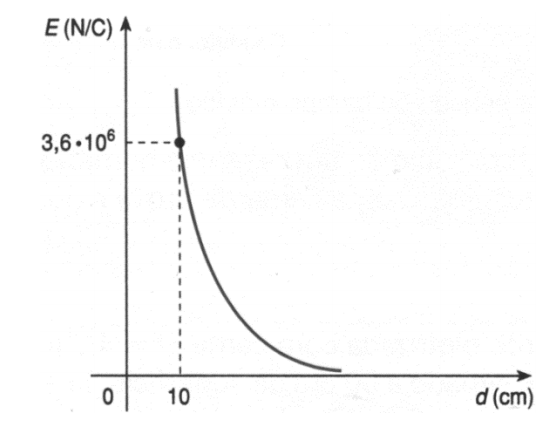
\includegraphics[scale=0.9]{imgs/q5.PNG}
			\end{center}
		\end{figure} 
		
		\newpage
		
		\question[10]
		O \textbf{potencial elétrico} no ponto $A$, do campo elétrico produzido por uma carga elétrica
		puntiforme $Q$, representado na figura \ref{figq6}, é $V_A = 3,0 \times 10^{3}$ volts. Determine:
		
		\begin{figure}[H]
			\label{figq6}
			\caption{Figura para a questão 6}
			\begin{center}
				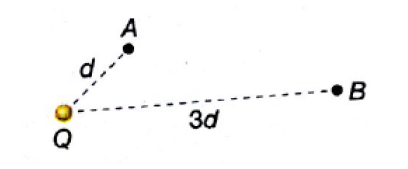
\includegraphics[scale=1.5]{imgs/q6.PNG}
			\end{center}
		\end{figure}
		
		\begin{parts}
			
			\item o \textbf{potencial elétrico} no ponto $B$.
			\vspace{4cm}
			
			\item a \textbf{diferença de potencial elétrico} entre os pontos $A$ e $B$.
			\vspace{4cm}
			
			\item o \textbf{trabalho realizado pela força elétrica} que age numa carga elétrica puntiforme $q = 1,0 \ \si{\micro}$C, quando deslocada do ponto $A$ ao ponto $B$.
			
		\end{parts}
		
		\newpage
		
		\question[10]
		\textbf{(MACKENZIE)} Entre os pontos $A$ e $B$ do trecho do circuito elétrico da figura \ref{figq7}, a ddp é $80$ V. Quanto vale a \textbf{potência dissipada} pelo resistor de resistência $4 \ \si{\ohm}$?
		
		\begin{figure}[H]
			\label{figq7}
			\caption{Figura para a questão 7}
			\begin{center}
				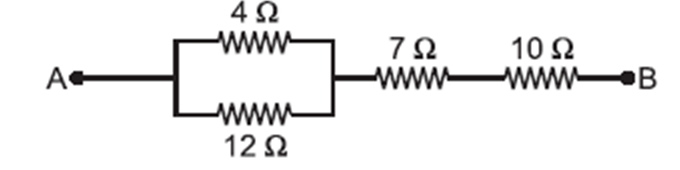
\includegraphics[scale=1]{imgs/q7.PNG}
			\end{center}
		\end{figure} 
		
		\vspace{3cm}
		
		\question[10]
		
		\textbf{(UNIUBE)} A \textbf{diferença de potencial} entre os pontos $A$ e $B$, do circuito da figura \ref{figq8}, é igual a $10$ V. Determine a \textbf{corrente} que passa pelo resistor de $6 \ \si{\ohm}$.
		
		
		\begin{figure}[H]
			\label{figq8}
			\caption{Figura para a questão 8}
			\begin{center}
				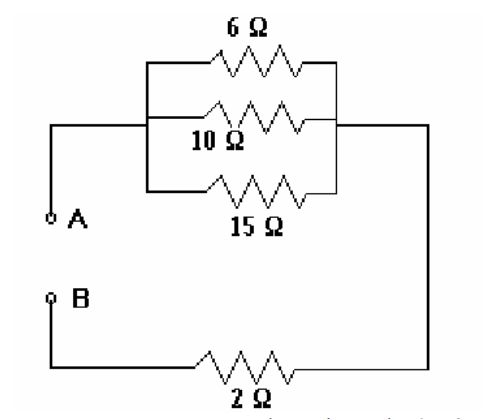
\includegraphics[scale=1]{imgs/q8.PNG}
			\end{center}
		\end{figure}
		
		\newpage
		
		
		\question[10]
		Dois \textbf{capacitores} de capacidades eletrostáticas $C_1 = 2 \ \si{\micro}$F e $C_2 = 6 \ \si{\micro}$F estão associados em \textbf{série} e ligados a uma fonte que fornece uma ddp constante de $20$ V. Determine: \\
		
		\begin{parts}
			
			\item a capacidade eletrostática do \textbf{capacitor equivalente}.
			\vspace{2.2cm}
			
			\item a \textbf{carga elétrica} de cada capacitor.
			\vspace{2.2cm}
			
			\item a \textbf{ddp} nas armaduras de cada capacitor.
			\vspace{3.2cm}
			
		\end{parts}
		
		
		\question[10]
		Dois \textbf{capacitores} de capacidades eletrostáticas $C_1 = 2 \ \si{\micro}$F e $C_2 = 6 \ \si{\micro}$F estão associados em \textbf{paralelo} e ligados a uma fonte que fornece uma ddp constante de $30$ V. Determine: \\
		
		\begin{parts}
			
			\item a capacidade eletrostática da \textbf{associação}.
			\vspace{2.2cm}
			
			\item a \textbf{carga elétrica} de cada capacitor.
			\vspace{2.2cm}
			
			\item a \textbf{energia elétrica} armazenada na associação.
			
		\end{parts}
		
		
	\end{questions}
\end{document}


